%
\section{Allgemeines}

MyCoRe ist ein Kernsystem, das alle Grundfunktionen von digitalen Bibliotheken und Sammlungen abdeckt.
Es kann als Basis f�r eigene Bibliotheksanwendung, aber auch f�r die Implementierungen einer ganz anderen Applikation zur Verwaltung multimedialer Objekte verwendet werden.
Dabei sollen eigene spezialisierte L�sungen insbesondere hinsichtlich der 
Datenmodellierung relativ schnell und einfach realisiert werden k�nnen. MyCoRe gestattet auch die Kopplung einzelner Installationen zu einem Verbund, was die Attraktivit�t erheblich erh�ht. Beispiele daf�r sind u. a. das MyCoRe-Sample oder das Papyrus-Projekt der Universit�ten Halle, Jena und Leipzig\footnote{\url{http://papyri.uni-leipzig.de}}.

\begin{figure}[h]
\begin{center}
\fbox{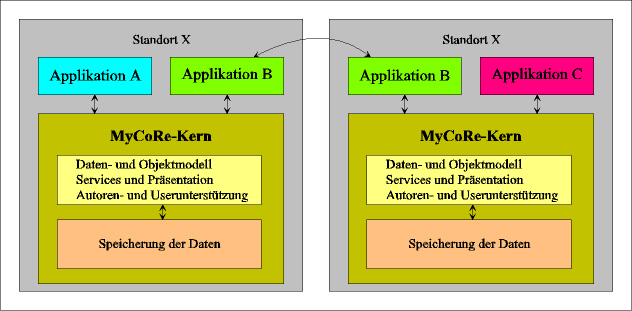
\includegraphics[scale=.8]{overview_kern_pic01.jpg}}
\label{overview_kern_pic01}
\caption{Grobes Schichtenmodell von MyCoRe}
\end{center}
\end{figure}

Auf dem obigen Bild ist dargestellt, wie MyCoRe-Anwendungen innerhalb eines Betreibers und aus der Sicht mehrerer Betreiber angelegt sind. In einer Einrichtung {\bf X} gibt es {\bf einen} MyCoRe-Kern pro Server, auf welchen mehrere Applikationen aufsetzen k�nnen. Dabei ist es auch m�glich, dass mehrere physische Anwendungen eine gemeinsame logische Anwendung (virtuelle datenbasis) darstellen. Dies erm�glicht gemeinsame Projekte verschiedener Einrichtungen auf der gleichen Basis.

Nachfolgend werden die Kernkomponenten mit einer Kurzbeschreibung der jeweiligen
Funktionalit"aten aufgef"uhrt.

\section{Dokumenten- und Personenmetadaten}
Das Metadatenmodell gew"ahrleistet die Mehrsprachigkeit aller relevanten Informationen.
Eine Reihe von Grundtypen f"ur die Metadatenmodellierung sind bereits im Kernsystem
implementiert.
Zu den angebotenen Grundtypen geh"oren.....

\section{Hierarchisches Klassifikationssystem}
\section{Internes Dateisystem}
Viele Systeme erm�glichen nur die Pflege und Bearbeitung von beschreibenden Daten (Metadaten)
zu Dokumenten und verwalten dar�ber hinaus nur einen Link auf die eigentlichen Dokumentvolltexte
auf einem Webserver. MyCoRe hingegen verwaltet nicht nur Metadaten, sondern auch die dazugeh�renden
Dateien selbst. Das bedeutet, dass die zu einem MyCoRe Objekt dazugeh�renden Dateien, wie z. B. die PDF- oder HTML-Version
eines Dokumentes oder das Foto einer Person bzw. Autors in das System importiert werden und 
dort verwaltet werden. 

MyCoRe besitzt zu diesem Zweck ein \mcridentifier{Internes Dateisystem} (Internal Filesystem, IFS), 
das Dateien,
Verzeichnisse und ihre Strukturen untereinander abbildet. Dieses Dateisystem verwaltet die Dateiinhalte
(Content) und beschreibende Informationen wie Dateiname, MD5 Pr�fsumme, Datum der letzten �nderung,
Verzeichnisstrukturen usw. Eine Programmierschnittstelle (API) erlaubt es, Dateien zu importieren,
zu ver�ndern oder zu l�schen, Dateien anhand von Pfadausdr�cken in einer intern abgebildeten 
Verzeichnisstruktur aufzufinden oder Verzeichnisinhalte zu sortieren. 

�ber das MyCoRe Command Line Interface k�nnen \mcridentifier{Derivate}, d. h. 
Dateib�ndel, die zu einem Dokument geh�ren, importiert oder aktualisiert werden. �ber ein Servlet
werden Dateien und Verzeichnisse im Browser angezeigt und ausgeliefert. In Vorbereitung ist auch
die M�glichkeit, Dateien interaktiv �ber den Browser in das System hochzuladen.

Die beschreibenden und technischen Daten zu Dateien und Verzeichnissen werden in einem \mcridentifier{FileMetadataStore}
gespeichert. Prinzipiell kann es f�r diesen Store verschiedene Implementierungen geben, derzeit ist
nur eine Implementierung f�r relationale Datenbanken realisiert, die sich z. B. mit MySQL oder DB2
nutzen l�sst.

Die Dateiinhalte dagegen werden getrennt davon in einem \mcridentifier{FileContentStore} gespeichert und verwaltet.
Derzeit gibt es f�nf Implementierungen eines FileContentStores, die je nacht Konfiguration des Systems auch
gleichzeitig eingesetzt werden k�nnen.

\section{Verteilte Suche und Schnittstellen}
\subsection{Verteilte Suche}
\subsection{Schnittstellen zu OAI, Z39.50, Webservices}

\section{Benutzer- und Zugriffsrechteverwaltung}
\subsection{Benutzerverwaltung}
\label{sec:LeistungsumfangUsermanagement} 
Im Subsystem Benutzermanagement wird die Verwaltung derjenigen Personen geregelt,
die mit dem System umgehen (zum Beispiel als Autoren Dokumente einstellen). 
Dazu bietet die Benutzerverwaltung insbesondere die M"oglichkeit, dass sich Benutzer 
und Benutzerinnen am System authentifizieren k"onnen.

Die Gesch"aftsprozesse einer Benutzerverwaltung wie zum Beispiel das Anlegen neuer 
Benutzer, das Setzen von Passw"ortern, die Aktivierung/Deaktivierung von Benutzern 
usw. erfordern unterschiedliche Privilegien. 
Das Benutzerverwaltungs-Komponente des MyCoRe-Projekts erm"oglicht eine detaillierte 
Rollen"ubernahme einzelner Personen auf Basis von Benutzergruppen, denen bestimmte
Privilegien zugewiesen werden k"onnen.
Das Privilegiensystem ist dabei frei definierbar (ein Satz grundlegender Privilegien
wird in der Dublin Core Beispielanwendung von MyCoRe mitgeliefert).
Zur Entlastung der Betreiber der digitalen Bibliothek ist es insbesondere m"oglich, 
dediziert administrative Privilegien an Kunden zu delegieren. 
Dies wird durch das Konzept von Gruppenadministratoren erm"oglicht, die besondere
Rechte f"ur die Verwaltung der Gruppenmitglieder besitzen.
Durch ein System von Regeln wird dabei gew"ahrleistet, dass sich ein Benutzer oder 
eine Benutzerin nicht selbst h"ohere Privilegien zuweisen kann, als vom jeweils 
"ubergeordneten Administrator festgelegt wurde.

Daten "uber Benutzer, Gruppen und Privilegien k"onnen aus XML-Dateien importiert
und in XML-Dateien exportiert werden.
Die Datenhaltung geschieht auf Basis einer SQL-Datenbank (z.B. IBM DB2, MySQL usw., je
nachdem, in welcher Softwareumgebung das MyCoRe-System betrieben wird).
Die Anmeldung am System geschieht "uber ein Servlet (MCRLoginServlet), auf das von
verschiedenen Stellen der Webanwendung hingewiesen werden kann. 
Dabei ist "uber ein MyCoRe-internes Session-Management gew"ahrleistet, dass die
Anmeldung "uber mehrere Transaktionen bzw. mehrere Anfragen an das System erhalten bleibt.
(Detaillierte Informationen hierzu finden Sie im 'MyCoRe Internal Design Guide'.)

\subsection{Verwaltung von Zugriffsrechten}
Macht Benno S"uselbeck...

\section{Benutzer- und Autoreninterface}



 
